\documentclass{article}

\usepackage{swiftnav}
\usepackage{pgfplots}
\usepackage{filecontents}


\usepackage{subcaption}

\usepackage{draftwatermark, array}
\SetWatermarkLightness{0.9}
\SetWatermarkText{Preliminary}
\SetWatermarkScale{1}
% Suppress numbers from section headings (but preserve PDF TOC).
\makeatletter
\renewcommand\@seccntformat[1]{}
\makeatother
\newcolumntype{$}{>{\global\let\currentrowstyle\relax}}
\newcolumntype{^}{>{\currentrowstyle}}
\newcommand{\rowstyle}[1]{\gdef\currentrowstyle{#1}%
  #1\ignorespaces
}
\newenvironment{mpar}{\par\noindent\minipage{\linewidth}}{\endminipage\par}
%\setlength{\skip\mpfootins}{2cm}
\renewcommand{\thempfootnote}{(\arabic{mpfootnote})}


% ---------------------------------------------------------------------------
\usepackage[section]{placeins}
\version{0.1}
\title{Piksi for UAV Aerial surveying}
\mysubtitle{RTK direct georeferencing with Swift Navigation's Piksi GPS receiver}
\author{Dennis Zollo, Rai Gohalwar}
\date{\today}

\ignorespaces

\begin{document}
\maketitle

\thispagestyle{firstpage}

\section{Abstract}
\label{sec:abstract}
This whitepaper presents using Piksi, a carrier phase differential GPS sensor, to georeference
 images from micro aerial vehicles (MAVs) in surveying use cases.
It presents both the sensor integration, data collection methods, and real-world surveying results
as processed by the PIX4D photogrammetry software.  Lastly, the value proposition of using RTK GPS
for aerial surveying is evaluated.
\tableofcontents
\newpage
\section{Overview}
\label{sec:Overview}
Due to the capability, low-cost, and popularity of micro aerial vehicles aerial surveying in industries such as precision agriculture, mining, and forestry is of great interest.

In a typical aerial surveying use-case, an aircraft is outfitted with a high-quality camera and
overflies an area of interest while capturing a series of images.  The images are then processed in
software to produce Digital Elevation Models (DEM's), Orthomosaics, and/or 3D point clouds which
can be used for photogrammetry applications, volumetric measurements, or crop health analysis to
provide business value for users.

Commercial software tools for photogrammetry have the ability to stitch together aerial images
through visual features with techniques such as Bundle adjustment.  Additionally, these software packages often
require rough location and orientation of the lense when the photo was taken.

To facilitate post-processing, most low-cost MAV control systems used for photogrammetry have
the ability to geotag photos as required by the processing software through Autonomous GPS combined
with MEMS sensors.  The typical sensor technology, however, combined with uncertainty in timing of the
camera's shutter, limits the precision and accuracy of geotagging information and therefore requires
post-processing software to rely heavily on image processing techniques. Additionally, large
amounts of sidelap and overlap between images and ground control points are often required to allow
post-processing software to utilize imagery information given the inaccuracy of the georeferencing
information.  Lastly, survey sites lacking in visual detail (such as agricultural land) or where
overlap is minimal (such as corridor mapping), often yield poor results with traditional techniques
and sensors.

It has been demonstrated that Carrier Phase Differential GPS (also called Real Time Kinematic (RTK)
GPS), can improve the location accuracy of georeferencing \cite{sensefly2}.  In the sections that
follow, we will demonstrate methods and results of using Swift Navigation's Piksi GPS Receiver to
geotag aerial photos for aerial surveying.  It is expected that precise and accurate geotagging
information can reduce the need for ground control points for typical survey missions, reduce the
amount of overlap and sidelap required, and improve the quality of ultimate photogrammetry
deliverables.

\section{Equipment and Setup}
\label{sec:equipment}
\begin{figure}[h]
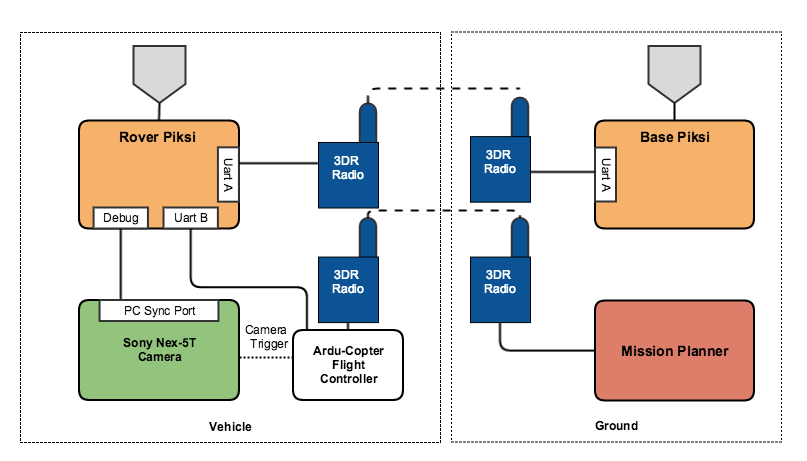
\includegraphics[width=7in]{images/flow_charts/uav_piksi_flow_chart.png}
\caption{Vehicle Diagram}
\label{figure:vehicle-diagram}
\end{figure}

\label{sec:equipment}
A camera, vehicle, and an image-tagging system using Piksi were developed to conduct experiments
with careful design considerations.  Available and low cost COTS equipment was chosen to highlight
that these results can be replicated without exotic or expensive equipment.  A Sony NEX-5t mirorrless DLSR Camera
with a fixed 20mm lense and a 16 MP CCID sensor was used as an imaging system. See table
\ref{cameraspecs} for detailed camera specifications. The application also required the
ability to electrically sense the shutter which was achieved through the use of a "Fotasy SANEX Hot
Shoe Adapter" Prontor/Compur (PC) socket for external flash synchronization.  The digital flash signal was
routed from the PC socket to the "external event" trigger feature of the Piksi receiver (pin 0 of Piksi's debug connector.)

The vehicle was designed and sized to carry the camera payload for a typical surveying mission.
While a fixed wing aircraft may be more applicable to surveying missions for their increased range,
a quadrotor configuration was chosen for low-cost and ease of implementation.  The test vehicle is
based on a 680 Tarot quad frame and uses four TigerMotor antigravity 4006 motors with 15 inch
propellers. The Pixhawk autopilot controls the aircraft and a 10.4Ah 6S battery pack powers. Fully
loaded the copter has a flight time of about 30 minutes. The Sony camera is attached pointing down
via a custom designed 3D printed a housing. Communication to both a base station Piksi and a UAV
Ground control station was accomplished via two 3D Robotics point to point radio modems. See table
\ref{table:vehicle-specs} for more information.

As an autopilot and flight controller, the Pixhawk flight controller running Arducopter version 3.3.2 was used.
A Ublox NEW 7N gps receiver functioned as a GPS sensor control (see table \ref{table:gps}.)
\begin{table}[]
\centering
\begin{tabular}{l^l}
\hline
\rowstyle{\bfseries}
Specification & Value \\ \hline
\rowstyle{}
Frame Type            & Quad-Rotor           \\ \hline
Frame                 & Tarot FY650          \\ \hline
Flight Controller     & 3DR Pixhawk          \\ \hline
Motors x 4            & T-Motor MN4006       \\ \hline
Motor Controllers x 4 & X-Rotor 40A OPTO     \\ \hline
Propellers x 4        & Tarot 1555 CF        \\ \hline
Batteries x 2         & Multistar 6S 5200mAh \\ \hline
Weight                & 2942 g               \\ \hline
\end{tabular}
\caption{Vehicle Specifications}
\label{table:vehicle-specs}
\end{table}

\begin{table}[]
\centering
\begin{tabular}{l^l}
\hline
\rowstyle{}
Primary GPS         & Piksi v2.3.1      \\ \hline
Primary GPS Firmware & v0.21 (STM) v0.16 (NAP)      \\ \hline
Secondary GPS       & U-Blox NEO 7N      \\ \hline
Primary Antenna     & Tellysman TW2412   \\ \hline
Secondary Antenna   & Taoglas gp.1575    \\ \hline
\end{tabular}
\caption{Vehicle GPS Specifications}
\label{table:gps}
\end{table}

\section{Method}
\label{sec:method}

\begin{table}[]
\centering
\begin{tabular}{l ^ l}
\hline
\rowstyle{\bfseries}
Specification & Value \\ \hline
\rowstyle{}
Camera                                                                & Sony Nex-5T        \\ \hline
Lens                                                                  & Sony SEL-20F28 (20mm)
\\ \hline
\begin{tabular}[c]{@{}l@{}}Weight\\ (with vehicle mount)\end{tabular} & 424 g              \\ \hline
Sensor                                                                & 16 MP: 4912 x 3264 \\ \hline
Hot shoe adapter \begin{tabular}[c]{@{}l@{}}Fotasy SANEX Hot Shoe Adapter \\(ASIN:
B00DE4T4E2)\end{tabular}  \\ \hline
\end{tabular}
\caption{Camera Specifications}
\label{cameraspecs}
\end{table}

\subsection{Site Selection and Ground Control}
A site was selected that combined high detail features such as structures and roadways with low detail features
grassland.  A series of 8 ground control points (GCPs) were surveyed using a Piksi receivers and a base station located
at a USGS survey marker about 2.2 Kilometers away.  One ground control point ended up outside of the survey area.
tSee figure \ref{fig:flightplan} for more information.

\begin{figure}
\centering
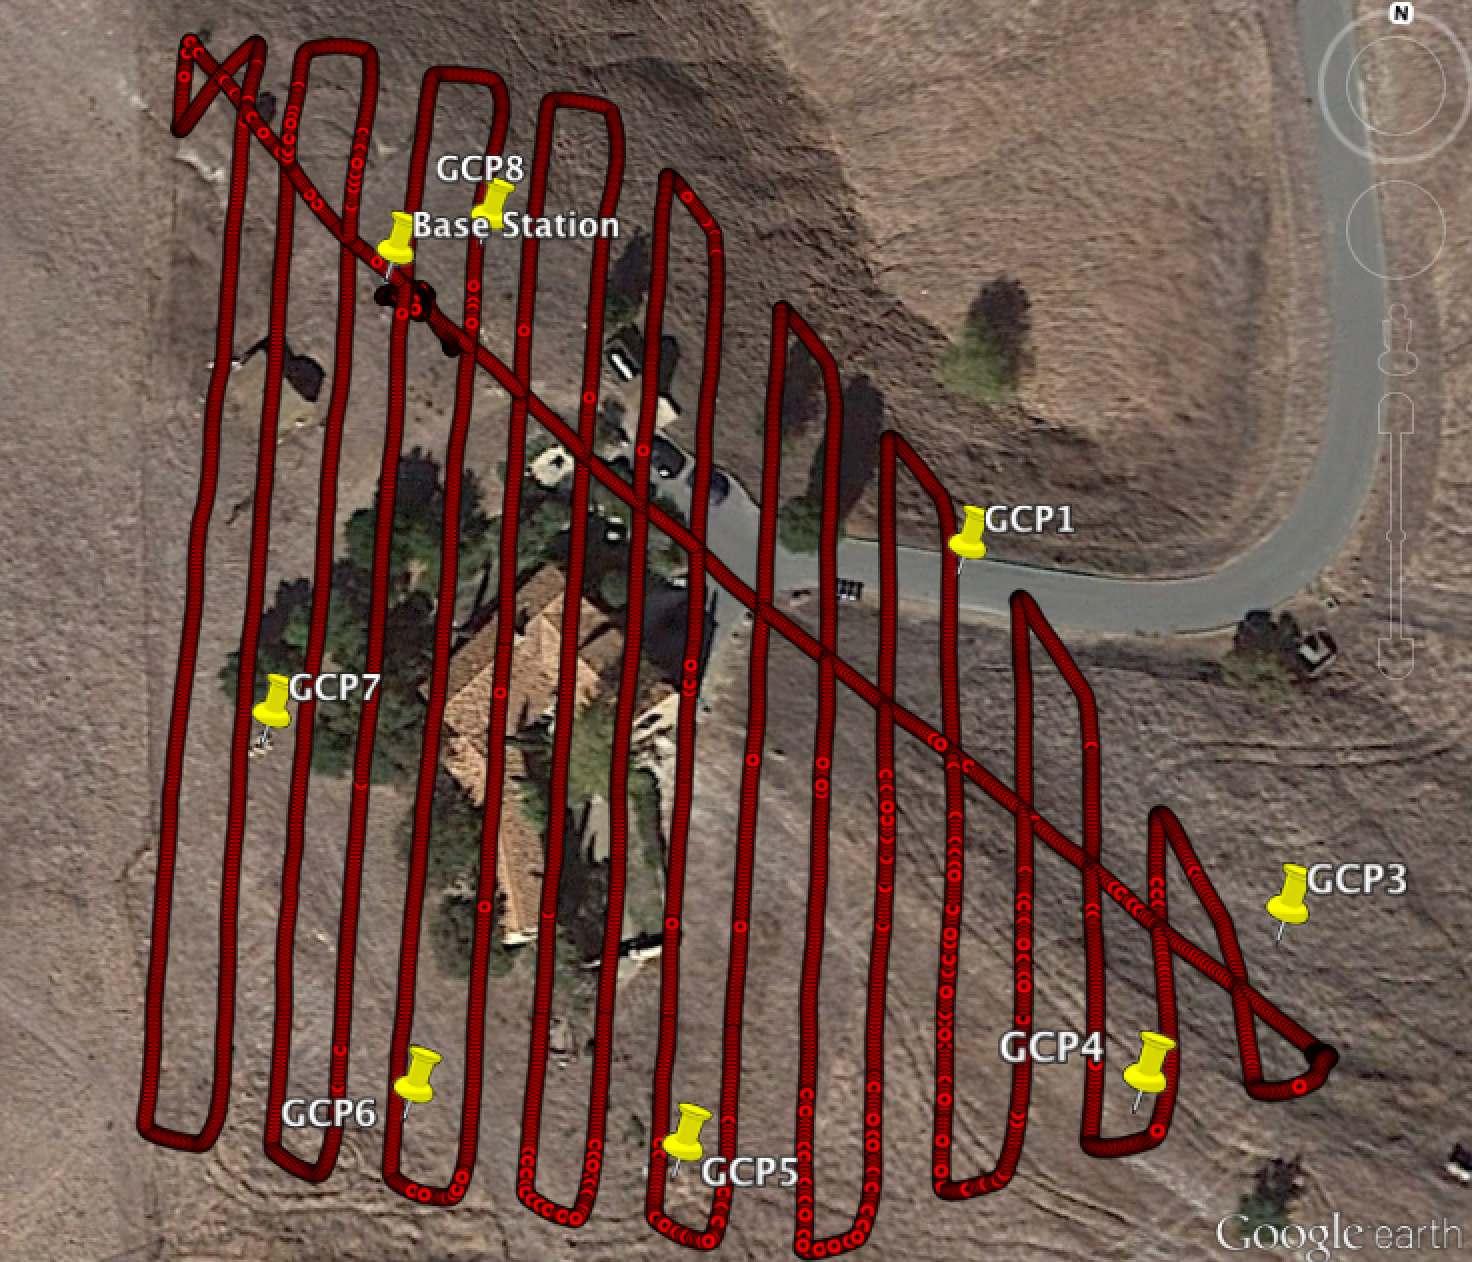
\includegraphics[width=5in]{images/flight_plan_gcp.png}
\caption{Flight plan visualization}
\label{fig:flightplan}
\end{figure}

\subsection{Mission Planning and Camera Configuration}
When conducting a surveying mission, it is very important to configure the vehicle, camera, and
flight parameters. To set flight parameters and other surveying parameters, Mission Planner GCS was
used. Mission Planner provided flight status during the mission and tools to convert user defined
surveying parameters (ground sampling distance, overlap, sidelap, area of interest, flight time and
camera direction) into an autonomous mission for Pixhawk.

The mission analyzed in this paper was designed with UAV surveying standards in mind. With a 75
percent overlap and 60 percent sidelap, the vehicle flew for approximately 22 minutes to capture
218 images. The copter in this mission was flown at 20m altitude which in theory gives a 2.37 mm
ground sampling distance (GSD). Pix4D reported an average GSD of 4.9 mm due to the terrain change and altitude variations of
the vehicle during the mission. Figure \ref{flightplan} shows the flight plan of the copter and the
locations of the ground control points.

To get the best quality possible, it was also necessary to configure the camera settings
appropriately. In order to avoid blur and compensate for the vibration and continuous movement of the vehicle
a constant shutter speed of 1/1250 sec was selected. The aperture settings and ISO were
selected automatically by the camera. This resulted in sharp and detailed images.

\section{Post-Processing Techniques}
\label{sec:postprocessing}
Post processing tools were developed in house for this project. Images captures from the camera
were not individually tagged. Instead, a file with the image names, Piksi geolocation coordinates,
orientation data (omega/phi/kappa) and accuracy (default of 5m horizontal and 10m
vertical) was generated. This file was consumed by Pix4D with the aerial images.

Figure \ref{postprocess} shows the basic layout of the post-processing routines as to allow the
methods to be reproduced.  Georeference-process.py is a top-level python script that processes the
data and generates a .csv file with image geolocations that can be consumed by Pix4d. There are
other scripts within that carry out individual tasks. Mavlink-decode.py extracts the piksi log file
(SBP JSON) from the dataflash BIN log file created by the Pixhawk. Interpolate-event.py linearly
interpolates the position data at the trigger points using the SBP log file. Query-mavlink.py is
used to interpolate attitude data at each shutter time. This attitude data is converted from aircraft Euler
angles to the "Image coordinate system" (omega/phi/kappa) specified by Pix4d in a Georeference-process.py
subroutine. All this data is then compiled into a csv file formate specified by Pix4d
with a Geolocation and camera attitude for each image.  All scripts are open-source and
available from Swift Navigation's Github repositories \url{http://github.com/swift-nav}
\subsection{Photogrammetry parameters}
In order to compare and analyze results from Pix4D, a total of 6 variations of settings and data
were selected for rendering as described in table \ref{table:postparams}.  The calibration method
column refers to whether the "Standard" calibration method in Pix4d or the "Accurate Geolocation
and Orientation" methods were used.  According to Pix4d help documentation, the "Accurate" setting
is "Optimized for project with very accurate image geolocation and orientation. This calibration
method requires all images to be geolocated and oriented."\cite{pix4d_support1}  The Included
images column refers to which images were used for post-processing (see section \ref{sec:overlap}
for more information)
The entire parameter space was repeated for the primary GPS (Piksi) and control GPS sensor (Ublox
sensor) as to make 12 total possible post-processing parameter sets.


\begin{figure}
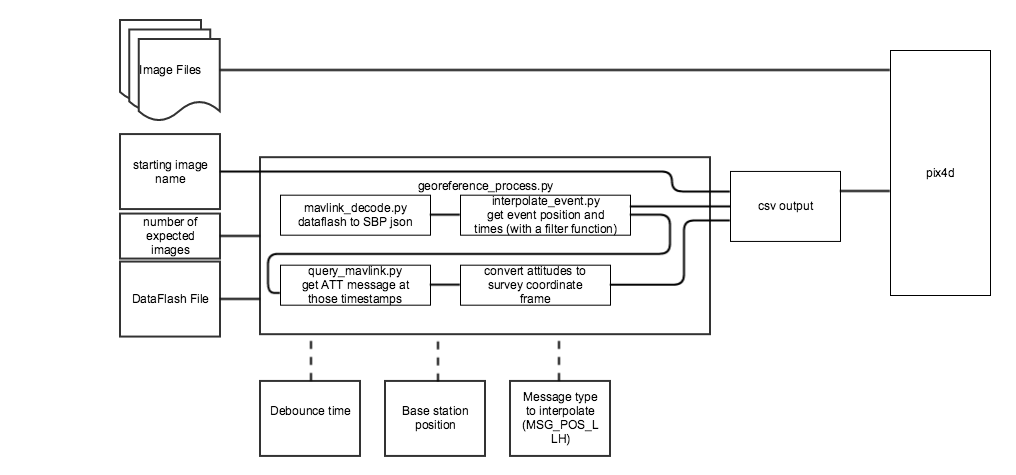
\includegraphics[width=7in]{images/flow_charts/uav_survey_processing_architecture.png}
\caption{Post Processing Architecture}
\label{postprocess}
\end{figure}

\begin{table}
\begin{tabular}{l ^ l ^ l ^ l ^ l ^ l} \\ \hline
\rowstyle{\bfseries}
Config & Description & Calibration Method & Included Images & GPS Sensor & Ground Control \\ \hline
\rowstyle{}
1  & Piksi RTK Std             & Standard  & All               & Piksi RTK (Fixed) & None \\ \hline
2  & Piksi RTK Std low sidelap & Standard  & Every Other Line  & Piksi RTK (Fixed) & None   \\
\hline
3  & Piksi RTK Std low overlap & Standard  & Every Other Image & Piksi RTK (Fixed) & None  \\ \hline
4  & Piksi RTK Std GCP         & Accurate  & All               & Piksi RTK (Fixed) & 7 GCPs \\
\hline
5  & Piksi RTK Acc             & Accurate  & All Images        & Piksi RTK (Fixed) & Nonoe \\ \hline
6  & Piksi RTK Acc GCP         & Accurate  & All               & Piksi RTK (Fixed) & 7 GCPs \\
\hline
7  & Ublox Std                 & Standard  & All               & Ublox             & None   \\
\hline
8  & Ublox Std low sidelap     & Standard  & Every Other Line  & Ublox             & None \\ \hline
9  & Ublox Std low overlap     & Standard  & Every Other Image & Ublox             & None  \\ \hline
10 & Ublox Std GCP             & Standard  & All               & Ublox             & 7 GCPs \\
\hline
11 & Ublox Acc                 & Accurate  & All               & Ublox             & None \\ \hline
12 & Ublox Acc GCP             & Accurate  & All               & Ublox             & 7 GCPs \\
\hline
\end{tabular}
\caption{Post processing parameterization}
\label{table:postparams}
\end{table}

\section{Results}
THe survey mission and the various post-processing techniques provided typical UAV survey results.  Most images were calibrated and stiched together to create survey outputs such as orthomosaics, digital elevation models, and point clouds.  In the section that follows, the resultant outputs are analyzed as to understand how improved GPS accuracy and different post-processing strategies can affect quality.
\begin{figure}
\centering
\renewcommand*\thesubfigure{\arabic{subfigure}}
\begin{subfigure}{.33\textwidth}
  \centering
  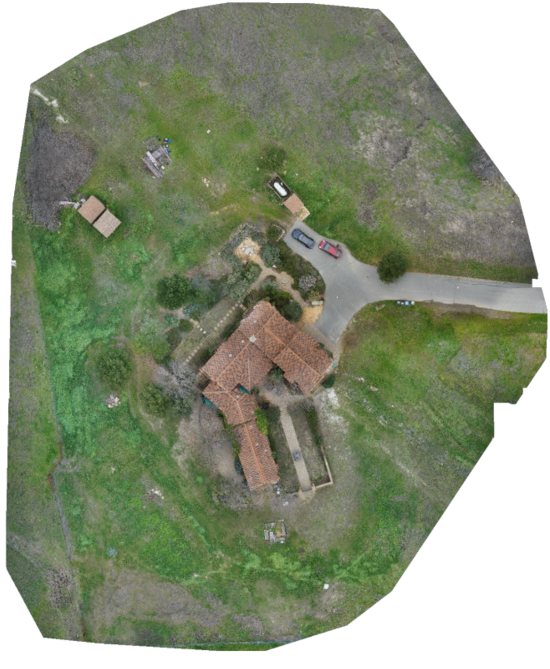
\includegraphics[width=.75\linewidth]{images/orthomosaics/p.png}
  \caption{Piksi all images}
  \label{fig:sub1}
\end{subfigure}%
\begin{subfigure}{.33\textwidth}
  \centering
  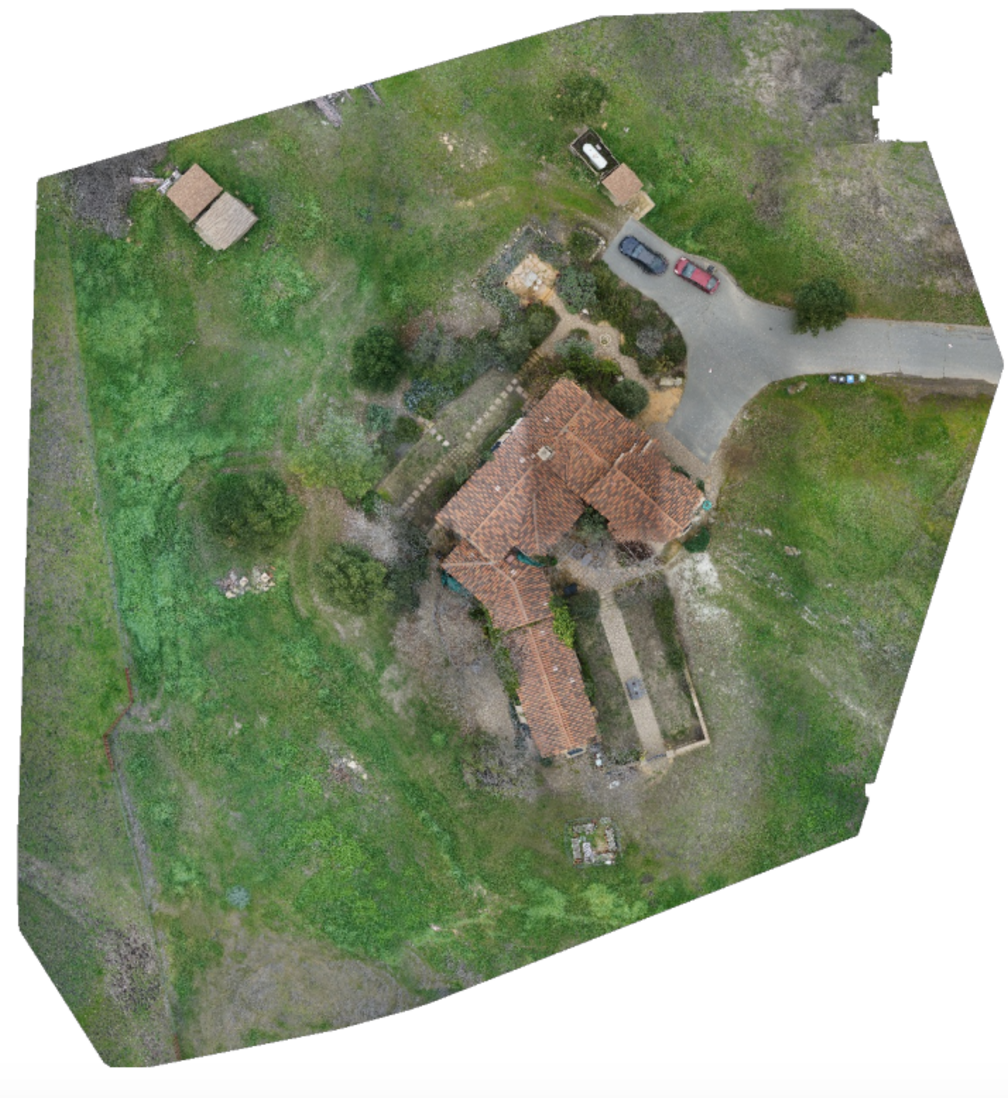
\includegraphics[width=.75\linewidth]{images/orthomosaics/p_every_other_line.png}
  \caption{Piksi every other line}
  \label{fig:sub2}
\end{subfigure}
\begin{subfigure}{.33\textwidth}
  \centering
  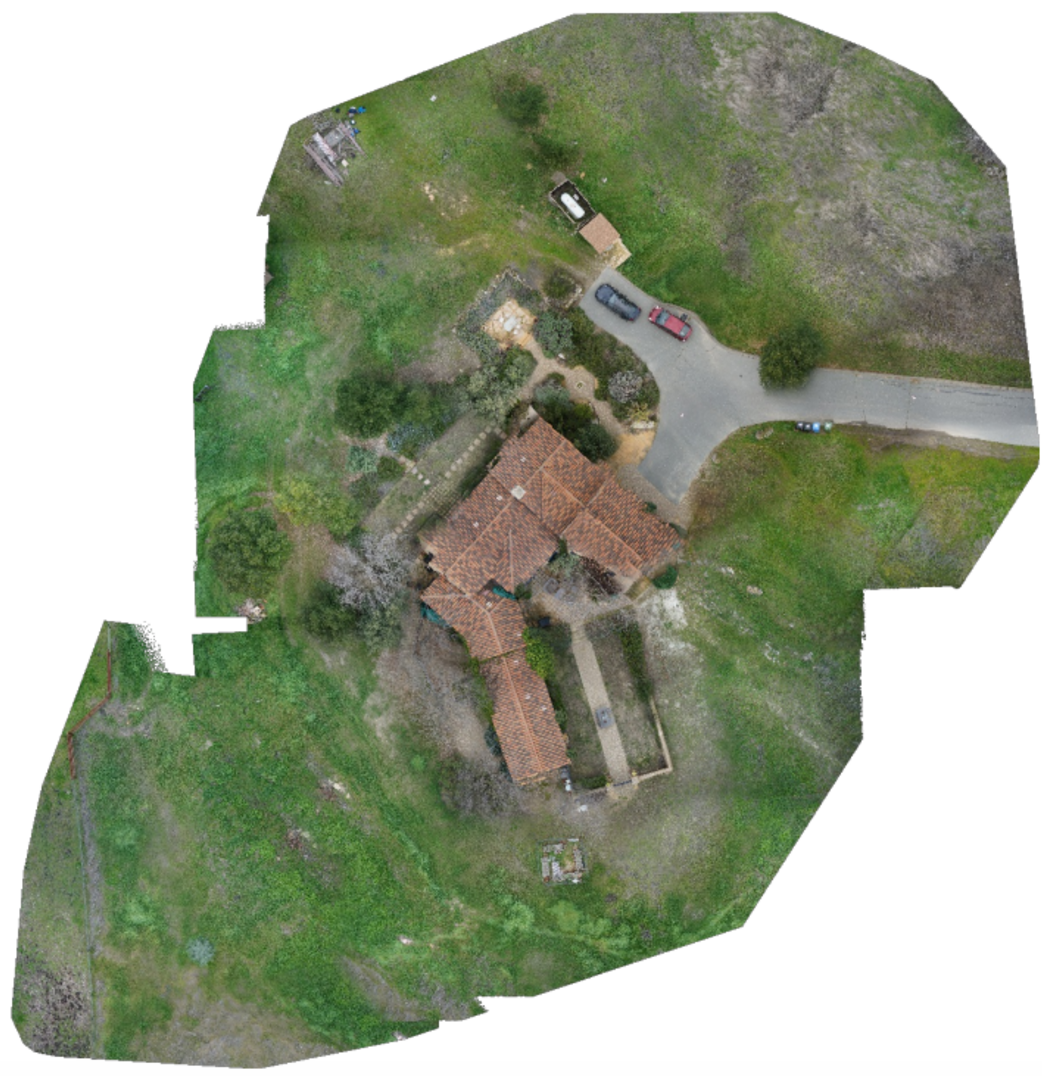
\includegraphics[width=.75\linewidth]{images/orthomosaics/p_every_other_image.png}
  \caption{Piksi Every Other Image}
  \label{fig:sub1}
\end{subfigure}%
\begin{subfigure}{.33\textwidth}
  \centering
  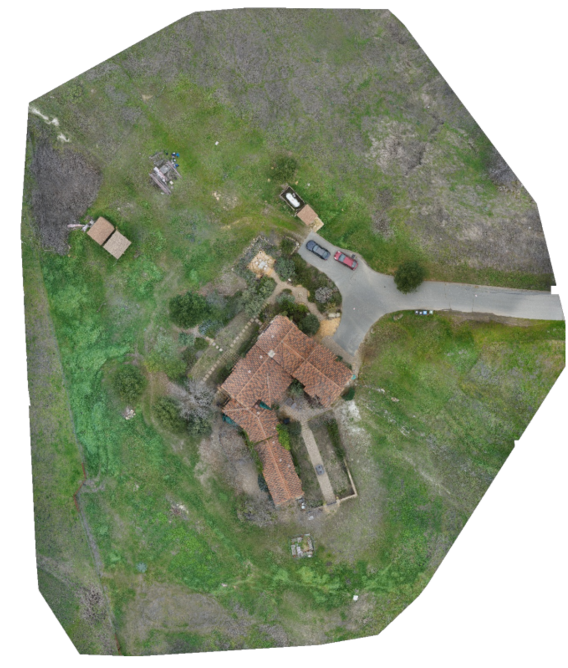
\includegraphics[width=.75\linewidth]{images/orthomosaics/p_gcp.png}
  \caption{Piksi with GCPs}
  \label{fig:sub1}
\end{subfigure}%
\begin{subfigure}{.33\textwidth}
  \centering
  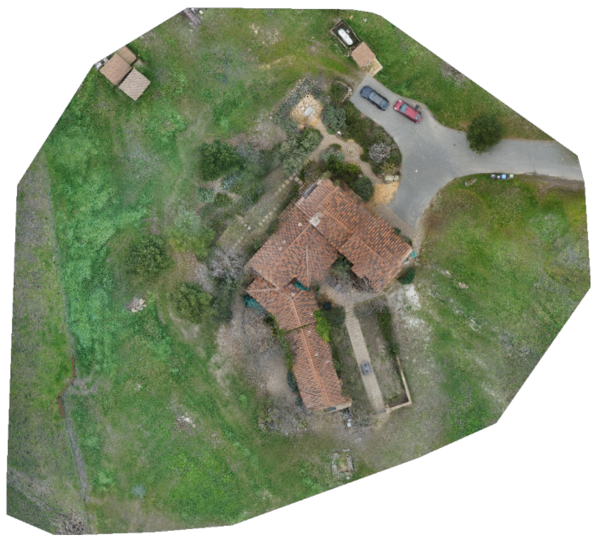
\includegraphics[width=.75\linewidth]{images/orthomosaics/p_accurate.png}
  \caption{Piksi Accuracy }
  \label{fig:sub2}
\end{subfigure}
\begin{subfigure}{.33\textwidth}
  \centering
  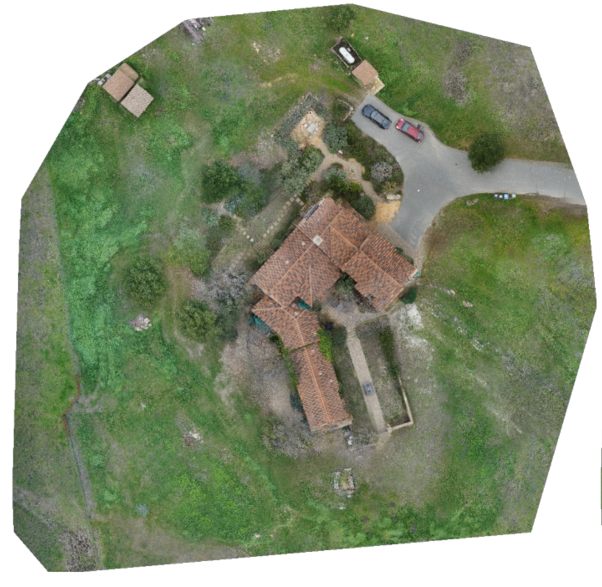
\includegraphics[width=.75\linewidth]{images/orthomosaics/p_gcp_accurate.png}
  \caption{Piksi Accuracy with GCPs}
  \label{fig:sub1}
\end{subfigure}%
\begin{subfigure}{.33\textwidth}
  \centering
  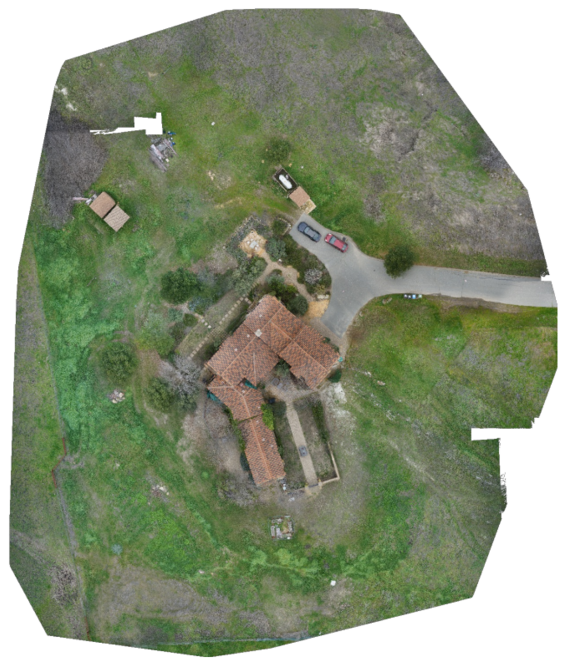
\includegraphics[width=.75\linewidth]{images/orthomosaics/ublox.png}
  \caption{Ublox All Images}
  \label{fig:sub1}
\end{subfigure}%
\begin{subfigure}{.33\textwidth}
  \centering
  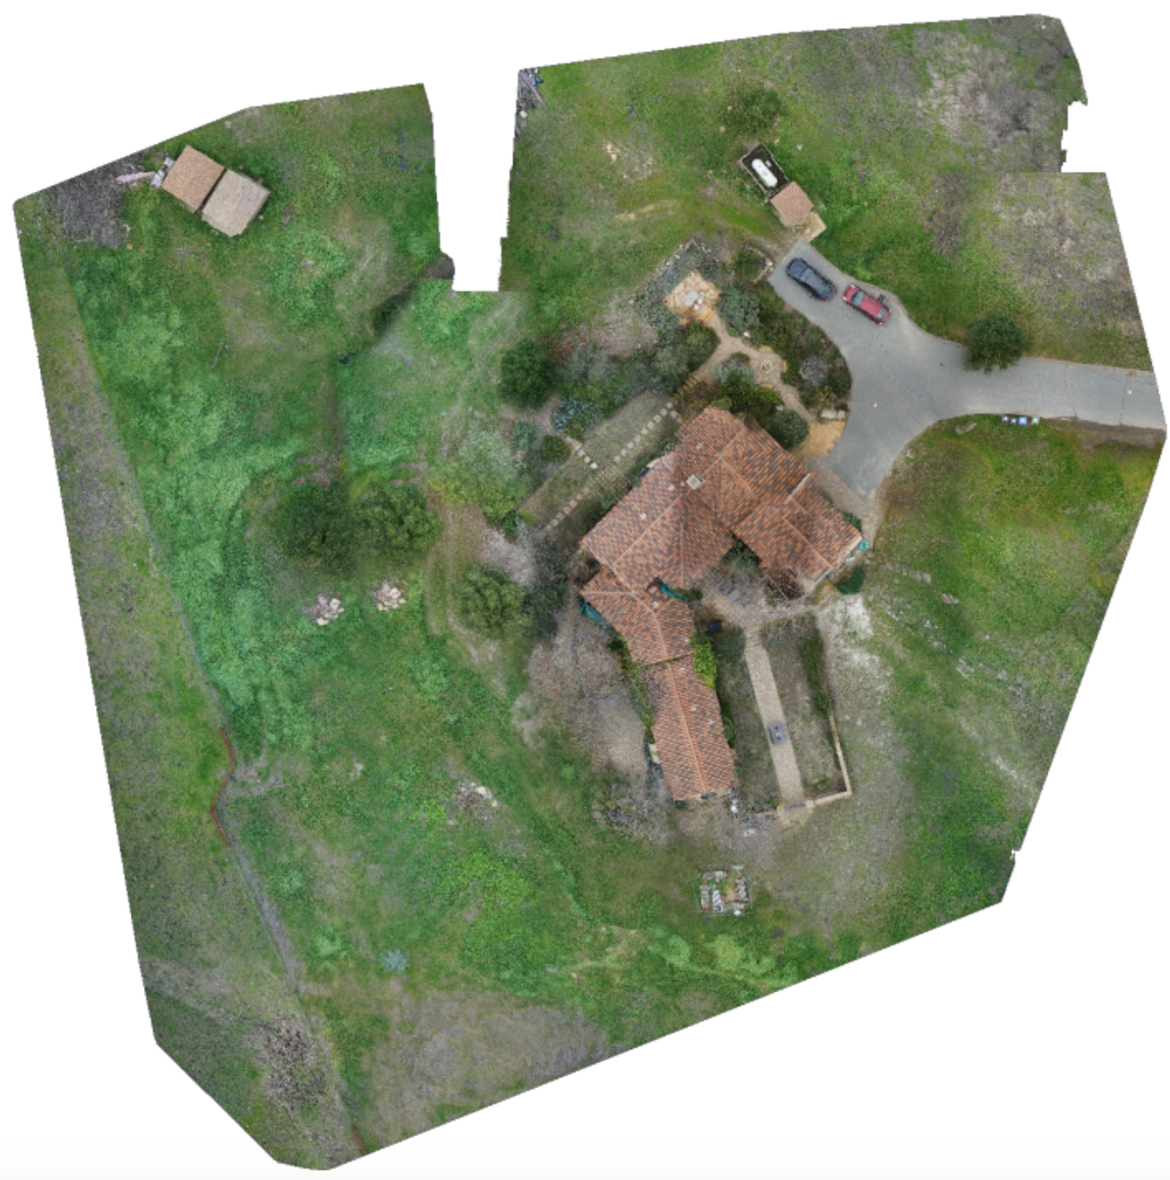
\includegraphics[width=.75\linewidth]{images/orthomosaics/ublox_every_other_line.png}
  \caption{Ublox Every Other Line}
  \label{fig:sub2}
\end{subfigure}
\begin{subfigure}{.33\textwidth}
  \centering
  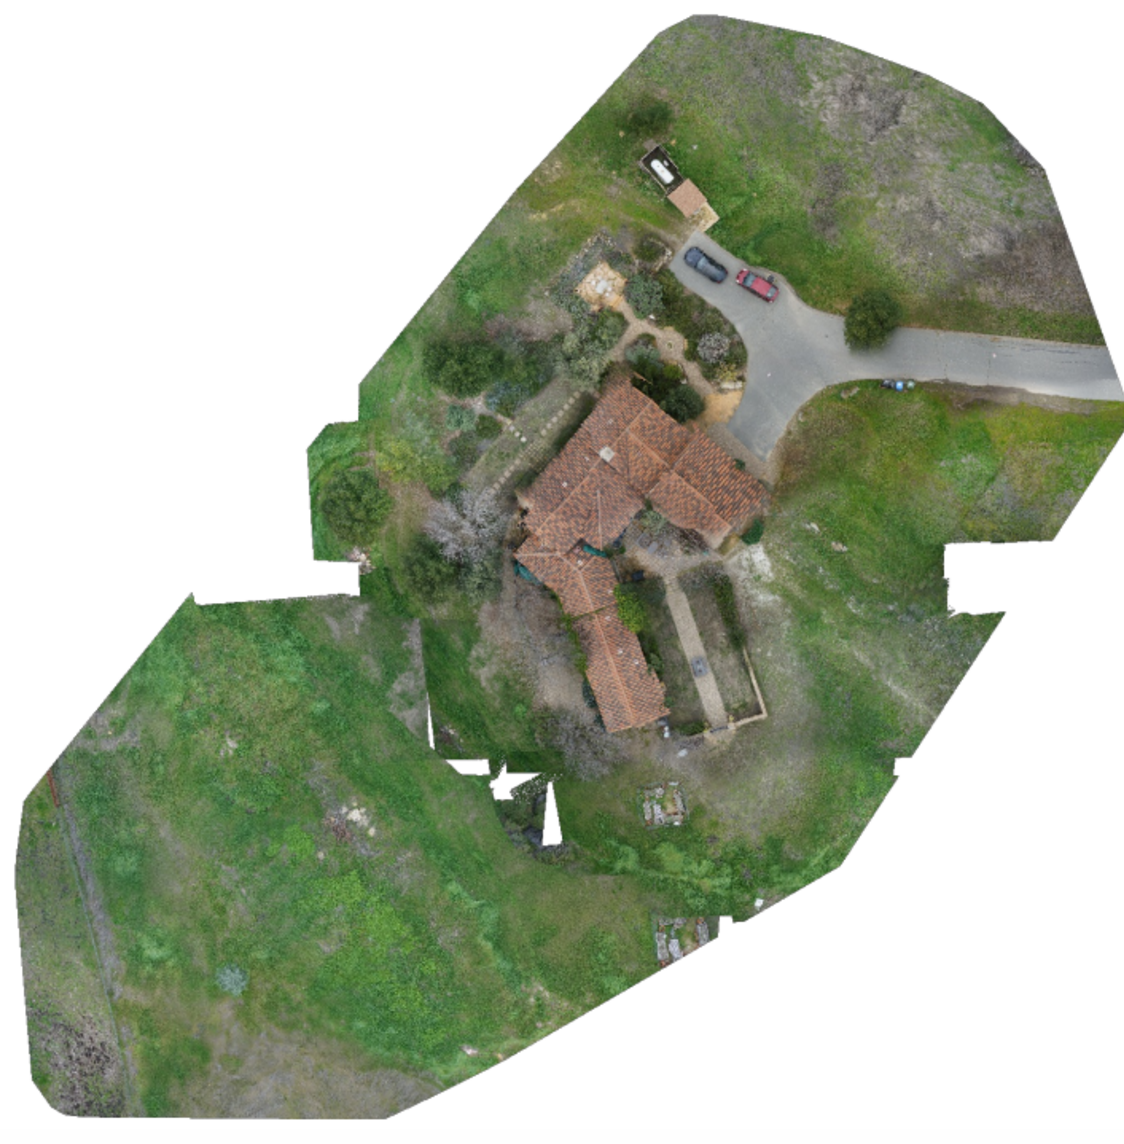
\includegraphics[width=.75\linewidth]{images/orthomosaics/ublox_every_other_image.png}
  \caption{Ublox Every Other Image}
  \label{fig:sub1}
\end{subfigure}%
\begin{subfigure}{.33\textwidth}
  \centering
  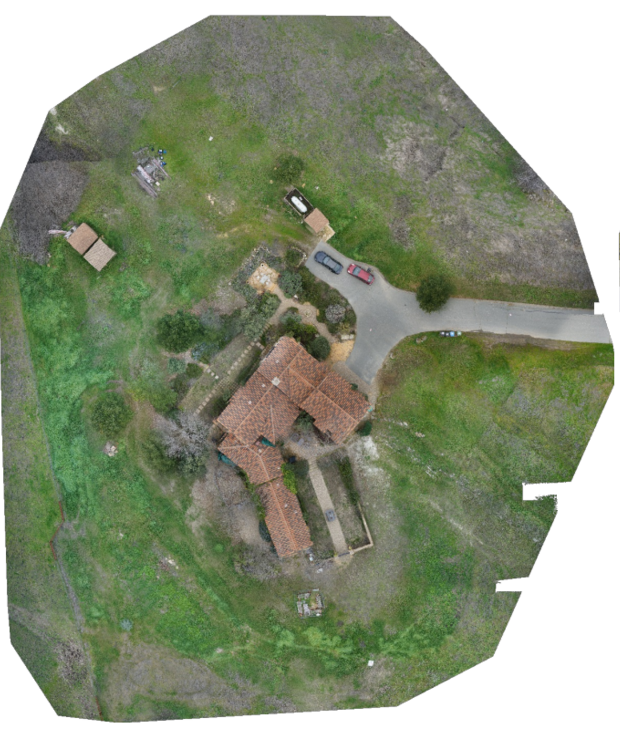
\includegraphics[width=.75\linewidth]{images/orthomosaics/ublox_gcp.png}
  \caption{Ublox with GCPs}
  \label{fig:sub1}
\end{subfigure}%
\caption{Orthomosaics of Different Configuration Renderings}
\label{ortho}
\end{figure}

\subsection{Accuracy}

Accuracy is very important when conducting a surveying mission. Ideally GCPs help post-processing
softwares refine the scale and help align the images better. Without GCPs, Pix4D is unlikely to
compute the true scale of the image unless image geo-referenceing information is very accurate. In
order to evaluate the ability to correctly scale an image, the distance between 2 GCP markers in
the post-processed image was used.  The calculated distances to the measured distance of 54.83
metres. There was little to no difference between the distance Piksi renderings showed compared to
the ublox renderings. The hypothesis is that, if the data is within a threshold, Pix4D does not
weight the image geolocation data and most of the stitching and scaling of the resultant point
cloud or orthomosaic comes from image processing.

A technical contact at PixD suggested using the "Accurate Geolocation and Orientation" calibration
methods in order to configure Pix4d to weigh more heavliy image geolocaiton information.

Configuration 5, 6, 11 and 12 were rendered using "Accurate Geolocation and Orientation" settings
in Pix4D.  It was expected that this calibration method would produce better orthomosaic and point
cloud results, but thi was not the case. Observing Table \ref{table:qualityreport} , both Piksi and
Ublox suffer from this setting. The RMS errors increase to a point that configuration 11 doesn't
produce DSM or orthomosaic and configuration 12 doesn't render at all. In Figure \ref{ortho} the
orthomosaics of Piksi clearly show the inaccuracy of renders with this setting compared to default
settings.

The only possible theory to explains this behavior is that the inaccuracy of the orientation data
dominates with this calibration method. Since the Pixhawk flight controller in the experiment has a
relatively low quality MEMS IMU, it cannot be expected to have highly accurate attitude
measurements during the flight.  Moreover it is possible that an error persisted in the conversion
from aircraft Euler angles to the surveying frame (omega/phi/kappa) required by Pix4d.  The exact
reason that this calibration method yielded poor results is unknown, but due to poor initial
results it was not pursued.

\begin{table}[]
\centering
\begin{tabular}{l ^ l ^ l ^ l ^ l} \hline
\rowstyle{\bfseries}
Configuration & X Error [m] & Y Error [m] & Z Error [m] & Image calibrated [percent]   \\ \hline
\rowstyle{}
1 & 0.185 & 0.136 & 0.274 & 84   \\ \hline
2 & 0.653 & 0.552 & 1.056 & 64    \\ \hline
3 & 0.847 & 1.182 & 1.202 & 59  \\ \hline
4 & 0.076 & 0.089 & 0.011 & 85    \\ \hline
5 & 0.556 & 0.619 & 0.989 & 99  \\ \hline
6 & 0.277 & 0.073 & 0.723 & 95   \\ \hline
7 & 0.202 & 0.840 & 0.563 & 82   \\ \hline
8 & 3.075 & 1.842 & 1.255 & 64   \\ \hline
9 & 2.191 & 3.028 & 1.897 & 57  \\ \hline
10 & 0.086 & 0.096 & 0.024 & 81   \\ \hline
11 & 0.500 & 0.625 & 0.959 & 99   \\ \hline
12 & \multicolumn{4}{^c}{Would Not Render} \\ \hline
\end{tabular}
\caption{Pix4D Quality Report Error and Camera Calibration Data}
\label{table:qualityreport}
\end{table}




\subsection{Overlap/Sidelap}
\label{sec:overlap}

Surveying missions are typically flown with high overlap to yield hight quality photogrammetry
results. Tools such as Pix4D are designed to favor image processing over geolocation information
due to lack of accuracy in the commonly used GNSS systems on micro UAVs. The hypothesis is that
with accurate geolocation data, the overlap percentage can be dropped without effecting the
performance.

The mission was designed to have an overlap of 75 percent and a side lap of 60 percent. The idea
behind these numbers was so that in post-processing we could eliminate entire lines from the flight
path and images and still be able to process the data. As shown in the configuration table
\ref{table:postparams} post-processing was performed after removing lines and after ignoring
every other image. The removal of lines would effectively halve the sidelap percentage.  The
removal of images would effectively halve the overlap percentage.

Figure \ref{figure:rmserror} shows the mean RMS errors extracted from Pix4D quality reports for
various configurations.As expected, both Piksi and Ublox experience significance increase in error
when lines and images are removed. That said, the error magnitude with Piksi's geolocation
information is smaller than that with Ublox. Additionally the number of images and the total area
that was successfully surveyed is larger when Piksi's RTK geolocation information is used to
georeference images. This analysis suggests that a more accurate GPS sensor can reduce the overlap
and sidelap necessary for successful image processing and thus increase the area that can be
surveyed in a given flight.


\begin{figure}
\centering
\begin{subfigure}{.5\textwidth}
  \centering
  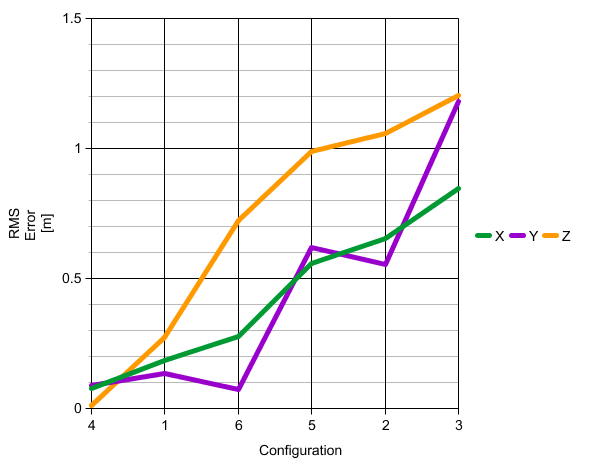
\includegraphics[width=1\linewidth]{images/piksi_rms_error.png}
  \caption{Piksi}
  \label{fig:sub1}
\end{subfigure}%
\begin{subfigure}{.5\textwidth}
  \centering
  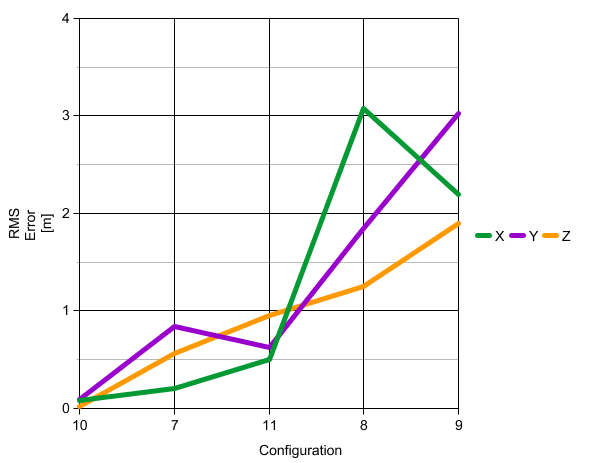
\includegraphics[width=1\linewidth]{images/ublox_rms_error.png}
  \caption{Ublox}
  \label{fig:sub2}
\end{subfigure}%
\caption{Piksi and Ublox RMS Error }
\label{figure:rmserror}
\end{figure}

\subsection{Initial accuracy estimate investigation}
One potential output to measure post-processing quality is the RMS errors reported by Pix4d
Software which come from the "Initial processing" step of the software.  Indeed, this paper, and
the marketing material of some vendors and other parts of the literature use this image processing
output as a key metric in evaluating the quality of geolocation surveying data.

In this analysis, however, the RMS errors values seemed highly affected by the image geolocation
"accuracy" estimates are initially provided to the software by the user as input.  This outcome was
peculiar and unexplained.  This odd relationship is presented in table \ref{table:accuracy}. The
table shows three identical post-processing runs where the only difference was the accuracy
estimate.  As this accuracy estimate decreased, the image location errors as reported in the Pix4d
quality report decreased as well.  This behavior suggests that the accuracy reported by Pix4d for
geolocation information is more an artifact of post-processing than representing something
physical.  For this paper the default initial accuracies were used as control for this behavior.  As
an additional note, in certain cases when these initial accuracy values are constrained to values
below the accuracy of the sensors used for geo-referenceing, the software is unable to perform
initial processing.


 % images processed  2d keypoints mean RMS Error [m] X RMS Error [m] Y RMS Error [m] Z

\begin{table}[]
\centering
\begin{tabular}{l ^ c ^ c ^ l ^ l ^c ^c ^c} \hline
\rowstyle{\bfseries}
Label & \multicolumn{2}{^c}{Initial Image Accuracy [m]}  & Images & 2d keypoints &
\multicolumn{3}{^c}{Mean RMS Error [m]} \\
&   X,Y & Z & processed (\%) & & X & Y & Z  \\ \hline
\rowstyle{}
a  &5   &10  &84  &5902  &0.184857  &0.136434  &0.273608 \\ \hline
b  &0.2 &1   &84  &5907  &0.126739  &0.097678  &0.163582 \\ \hline
c  &0.1 &0.2 &84  &5887  &0.061538  &0.06066   &0.111367 \\ \hline
\end{tabular}
\caption{Initial Accuracy Estimate Data}
\label{table:accuracy}
\end{table}

\section{Conclusions}
Conclusions here
\subsection{Issues}
\subsection{Next Steps}
Surveying a crop field and other landmarks is a very daunting task. It requires expensive equipment 
and skills to understand and produce valuable data. MAVs bring all these tools to the people in an 
affordable and easy to understand fashion. In attempt to prove the benefit of accurate geotags for 
aerial surveyed data, a wide room of improvement was realized. First and foremost, one of the 
limiting factors for this project was the closed nature of Pix4D. Many of the results could have 
been better explained if Pix4D's rendering process was explained. Features such as initial accuracy 
and orientation inputs(omega/phi/kappa) had unexplained roles in the rendering process. For future 
development, either switching to a different post processing tool (Agisoft PhotoScan or Visual 
Surveyor) or understanding Pix4D deeply would be of best choice. 



\begin{thebibliography}{9}
\bibitem{sensefly1}
Strechha,  Christophe (2011). "The Accuracy of Automatic Photogrammetric Techniques on Ultra-Light
UAV Imagery." \texit{UAV-g 2011 - Unmanned Aerial Vehicle in Geomatics.} Zürich, CH, September
14-16, 2011
\bibitem{sensefly2}
A. Roze, J-C. Zufferey, A. Beyeler, A. McClellan \textit{eBee RTK Accuracy Assessment}.
Retrieved from
\url{https://www.sensefly.com/fileadmin/user_upload/sensefly/documents/eBee-RTK-Accuracy-Assessment.
pdf}
\bibitem{pix4d_support1}
"Menu Process Processing Options... 1. Initial Processing Calibration." Pix4d. Retrieved March 24,
2016, from \url{https://support.pix4d.com/hc/en-us/articles/205327965#label2&gsc.tab=0}
\end{thebibliography}
\thispagestyle{lastpage}
\end{document}
